\documentclass[a4paper, 11pt]{article}
% For UTF-8 encoding
\usepackage[utf8]{inputenc}
% For proper hyphenation etc.
\usepackage{babel}
% For clickable links
\usepackage{hyperref}
% Set page margins
\usepackage[top=2cm, bottom=2cm, left=2.5cm, right=2.5cm]{geometry}
\usepackage{amssymb}
\usepackage{amsmath}
\usepackage{tikz}
\usepackage{pgfplots}
\usetikzlibrary{calc,shadings}
\usetikzlibrary{positioning}
\usepackage{amsthm}
\usepackage{color}
\usepackage{algorithm,algorithmic}
\usepackage[singlespacing]{setspace}

%Definitions
\newtheorem{mydef}{Definition}
\newtheorem*{remark}{Remark}
\newtheorem{example}{Example}
\newtheorem{lemma}{Lemma}
\newtheorem{theorem}{Theorem}
\newtheorem{corollary}{Corollary}
\newtheorem{proposition}{Proposition}

\makeatletter
\renewenvironment{quotation}
{\list{}{\listparindent=1.5em
		\itemindent=0pt
		\parsep\z@ \@plus\p@}%
	\item\relax}
{\endlist}
\makeatother

\newenvironment{customlegend}[1][]{%
	\begingroup
	% inits/clears the lists (which might be populated from previous
	% axes):
	\csname pgfplots@init@cleared@structures\endcsname
	\pgfplotsset{#1}%
}{%
	% draws the legend:
	\csname pgfplots@createlegend\endcsname
	\endgroup
}%

%definitions
\def\addlegendimage{\csname pgfplots@addlegendimage\endcsname}
% definition to insert numbers
\pgfkeys{/pgfplots/number in legend/.style={%
		/pgfplots/legend image code/.code={%
			\node at (0.295,-0.0225){#1};
		},%
	},
}

\usepackage{fancyhdr}

\newcommand{\HRule}[1]{\rule{\linewidth}{#1}}
\setcounter{tocdepth}{5}
\setcounter{secnumdepth}{5}

%-------------------------------------------------------------------------------
% TITLE PAGE
%-------------------------------------------------------------------------------

\begin{document}
	
	\title{ \normalsize \textsc{Seminar: Selected Topics in Logic and Verification }
		\\ [2.0cm]
		\HRule{0.5pt} \\
		\LARGE \textbf{\uppercase{A Summary on:\\
			A Pivoting Algorithm for Convex Hulls and Vertex Enumeration of Arrangements and Polyhedra}
		\HRule{1pt} \\ [0.5cm]
		\normalsize September 30, 2020 \vspace*{5\baselineskip}}
	
	\date{Summer semester 2020}
	
	\author{
		Tilman Hinnerichs \\
		Matrikelnummer: 4643427 \\ 
		Technische Universität Dresden\vspace{1cm}\\
		Tutor: Dr. Florian Funke }}
\maketitle
\newpage
\begin{abstract}
	
\end{abstract}

\tableofcontents

\newpage

\section{Introduction}
This summary outlines the approach from Avis and Fukuda to the Vertex Enumeration problem mollified with various references to basic concepts such as the \textsc{Simplex} algorithm.\medskip

The Vertex Enumeration Problem (VEP) is one of the most fundamental problems in computational geometry and has applications in fields such as computational biology and quantum physics. We will motivate solving the VEP with a more daily example later on.\medskip

The paper \glqq A Pivoting Algorithm for Convex Hulls and Vertex Enumeration of Arrangements and Polyhedra\grqq{} was written by David Avis and Komei Fukuda. It was published in 1992 in the journal \glqq Discrete \& Computational Geometry\grqq{} and is regarded as one of the most cited papers in this field with a number of 751 citations (as of 26.09.2020, according to Google Scholar). As a non-book, non-survey paper publication in such a specific field of research, this can be considered a fairly high amount of citations, emphasizing its importance.\medskip

We will thus follow a similar outline by first introducing polyhedra and arrangements, and the VEP on those. We then observe linear optimization problems and how they can be solved by the Simplex algorithm.

\section{Polyhedra and Arrangements}
In this first section we will introduce the needed notations and basics for the Vertex Enumeration Problem (VEP). At first, we will have to clarify the terms and concepts of the \textit{vertex} and \textit{polyhedra}.

\begin{mydef}(Polyhedron)\medskip
	A \textit{convex polyhedron} $G$ is defined as
	\begin{equation}
		G = \{ x\in \mathbb{R}^n: Ax+b\geq 0 \}\text{
			for some }A=(a_{ij}) \in \mathbb{R}^{m\times n}\text, b \in \mathbb{R}^m
	\end{equation}
\end{mydef}

This definition states that the set of points is constrained by a set of $m$ linear inequalities with $n$ variables that are basically hyperplanes in the \textit{n} dimensional space. In general and without loss generality, we assume that $G\neq\emptyset$, if not stated otherwise. In the following we will abbreviate \textit{convex polyhedra} simply as \textit{polyhedra}. \medskip

An \textit{arrangement of hyperplanes} or \textit{arrangement} for short, is a decomposition of the given underlying space using a set of hyperplanes. As both concepts are fairly similar, we will not explicitly list \textit{arrangements} in every definition, as every following statement holds for both polyhedra and arrangements. If that is not the case, arrangements will be named separately.\medskip

As the convex property is crucial for this approach to work, we will define it using convex combinations.
\begin{mydef}(Convex combination)\medskip
	
	Let $x_1, x_2, \dots, x_n\in\mathbb{R}^n$ be a finite set of points. A convex combination is a point $y\in\mathbb{R}^n$ of the form 
	\begin{equation*}
		y = a_1x_1 + a_2x_2 + \dots + a_nx_n
	\end{equation*}
	while $a_1, \dots, a_n\in\mathbb{R^+}$, and
	\begin{equation*}
		a_1 + \dots + a_n = 1
	\end{equation*}
	
	A convex combination is a linear combination.
\end{mydef}
Based on this definition we can further describe the constraints to our polyhedra and arrangements.
\begin{mydef}
	A set is called \emph{convex} if it contains all convex combinations of its points.
\end{mydef}
This also applies to polyhedra and arrangements.
\begin{mydef}
	For a given set of points, the convex hull is the set set of all convex combinations of these points.
\end{mydef}

\begin{figure}
	\centering
	\includegraphics[width=0.3\textwidth]{Convex_combination_illustration.svg.png}
	\label{convexComb}
	\caption{Visualization for convex combinations depicting the convex hull of $x_1, x_2, x_3$. $x_1,x_2,x_3$ are vertices of this polygon. All points within the triangle including $P$ are convex combinations of the vertices. All points outside like $Q$ are not convex combinations. }
\end{figure}

Both concepts are visualized in figure \ref{convexComb}.

In order to fully understand the last part of the title we additionally have to clarify the term \textit{vertex}, which we do by the following definition.

\begin{mydef}(Vertex)\medskip
	\label{vertex}
	Let $G$ be a polyhedron. A point $v\in G$ is called a \textit{vertex} of a set $G$ iff there are no two other points $a,b\in G$ such that
	\begin{equation}
		v=\lambda_1 a + \lambda_2 b
	\end{equation}
\end{mydef}

In order to make this definition a little more specific with regard to the definition of a polyhedron, we will introduce our first lemma.

\begin{lemma}\label{corollary1}\cite{introtoAlg}\medskip
	Let polyhedron be described by $A,b$. Let $m:=rank(A)$.\medskip
	A point $v\in G$ is a \textit{vertex} of $G$ iff it is the unique solution to a subset of $m$ inequalities of $G$ solved as equations. 
\end{lemma}

\section{The Vertex Enumeration Problem}
We are now ready to introduce the VEP itself with the following definition.
\begin{mydef}(Vertex Enumeration Problem)\medskip
	For a given polyhedron/polyhedron or hyperplane arrangement $G$ determine all vertices of the object given its formal representation. 
\end{mydef}

\begin{theorem}(Complexity of the VEP)\medskip
	Given a polyhedron $G$ and a list of vertices $V$, deciding whether $V$ contains all vertices of $G$ exactly once is NP-hard.\cite{Khachiyan}
\end{theorem}

The VEP is dual to the \textit{Facet Enumeration problem} (FEP), that is finding all facets of a convex hull for a given set of points. The solution to the dual problem also yields the solution to the primal problem, too. We will introduce the term of duality in the following chapter.\medskip

While these definitions lack the ability to intrinsically motivate the applicability of this very problem, we will introduce a fairly simple example, which was taken and simplified from Avis' lecture notes.
\begin{example}(All meals for 1 Euro)\medskip
	Let u
	s assume we are on a diet and additionally quite poor or minimalistic. Thus, we would like to plan our future meals, such that they only contain 3 different ingredients. Additionally, we would love to have sufficient nutrition intake, where we will only consider energy, protein and calcium intake.\medskip
	Our decision is also constrained by the fact that we will only have 1 Euro per day, and can also endure just up to a certain amount of each ingredient, in order not just eat dry oatmeal all day long.\medskip
	The values describing our problem are given in the following table:\medskip
	\begingroup
	\def\arraystretch{1.5}
	\begin{tabular}{|p{0.5cm}|l|p{2cm}|p{1.5cm}|p{1.5cm}|p{1.5cm}|p{2cm}|}
		\hline
		Var&Food type&Energy (kcal/100g)&Protein (g)&Calcium (mg)&Price (Euro cents)&Maximum\\
		\hline
		$x_1$&Oatmeal&250&15&40&10&500g\\
		$x_2$&Milk&80&4&130&4&1000g\\
		$x_3$&Dresdner Stollen&340&7&30&20&200g\\
		\hline
		&\textbf{Min. daily}&\textbf{2000}&\textbf{55}&\textbf{800}&&\\
		\hline
	\end{tabular}
	\endgroup\medskip
	
	The variables $x_1, x_2, x_3$ each denote the amount of each ingredient in 100g.
	
	This example problem can be expressed by the following system of inequalities with $Ax+b\geq0$. As visualisation of this can be found in the appendix.\medskip
	
		\begin{equation*}
		A = \begin{bmatrix}
			350&80&340\\
			15&4&7\\
			40&130&30\\
			-10&-4&-20\\
			-1&0&0\\
			0&-1&0\\
			0&0&-1\\
		\end{bmatrix},
		x = \begin{bmatrix}
			x_1\\x_2\\x_3\\
		\end{bmatrix},
		-b = \begin{bmatrix}
			2000\\
			55\\
			800\\
			-100\\
			-5\\
			-10\\
			-2\\
		\end{bmatrix},
		\begin{pmatrix}
			Energy\\
			Protein\\
			Calcium\\
			Price\\
			x_1Max\\
			x_2Max\\
			x_3Max\\
		\end{pmatrix}
	\end{equation*}
\end{example}

By solving the VEP, we yield all vertices of the corresponding polyhedron, that is all points that cannot be written as convex combinations of two other points. Inverting this very statement, all other points within $P$ are convex combinations of at least two other points. More specifically we are able to rewrite each point within $P$ as convex combinations of vertices of $P$. Thus, if we find all vertices of the given arrangement of linear inequalities, we can produce infinitely many food combinations by randomly choosing a convex combinations of the given vertices. However, we still have to find these vertices.\medskip

In history there have been various approaches to the VEP, that can be classified into two categories. First, there are the so called \textit{Pivot based} methods, where this very method can be placed, too. These methods rely on traversing along the vertices using so called \textsc{Simplex} tableaus, which we will introduce in the following chapter. The second method is called \textit{Fourier-Motzkin} or \textit{double description} method\cite{Motzkin}. These methods yield the vertices by successively adding hyperplanes and keeping track of the remaining possible vertices. The double description method in fact solves the dual problem that is FEP. 

\section{Linear Programs}
\subsection{What is a Linear Optimization Problem?}
While linear optimization problems are in general not necessary in order to solve the VEP with a pivot based method, it was utilized for this very approach. Additionally it gives us the chance to discuss and introduce some definitions and theorems that underline its simplicity and effectiveness. In the following we will use the terms \textit{linear program}(LP) and \textit{linear optimization problem} interchangeably.\medskip

\begin{mydef}
	Let $ G \subseteq \mathbb{R}^n$ be a polyhedron and $ c \in \mathbb{R}^n$. Then a problem of the form \medskip
	\vspace{0.15cm}
	\begin{quotation}
		$ z = f(x) = c^Tx \rightarrow min\hspace{1cm} with\ x \in G$
	\end{quotation} 
	is called a \emph{linear} optimization problem.
\end{mydef}

Hereby $G$ describes the feasible space as a set of $n$-dimensional vectors, while the objective function is denoted with $f:P\rightarrow\mathbb{R}$, which maps the vectors into the real numbers. Additionally, we can easily see the type of optimization, here minimization, while a maximization problem is possible,too. Without loss of generality we will only consider minimization problems here. If both objective function and all inequalities defining the feasible space are linear, we also call the program linear. \medskip

Furthermore, we are able to add a statement about the \textit{standard form} of linear programs. \medskip
\begin{lemma}\cite{introtoAlg}
	All finite dim. linear optimization problems can be written in the following form:\medskip
	\begin{equation}
		\label{standardform}
		z = f(x) = c^T x \rightarrow min \hspace{1cm} with\ x \in G:=\{x \in \mathbb{R}^n: Ax \geq b, x \geq 0\}
	\end{equation}
	with $A\in \mathbb{R}^{m\times n}$, $b\in\mathbb{R}^m$, $x\geq 0$.	Additionally, let $rank(A)=m$ and $m< n$.\\
	We call this form the \textit{standard form}.
\end{lemma}
The finite dimensionality is expressed with regard to the amount of variables, and thus the width of both objective function and coefficient matrix. \medskip

Hereby, the notation $x\geq0$ with $x\in \mathbb{R}$ describes the expression $x_j\geq 0$ for every $j=1,2,\dots,n$.\medskip 
Please note that we naturally do not have any objective function in the original VEP formulation. For now, let us assume that we do have a any linear objective function $f$ given. We will discuss this issue in further detail later on.\medskip
After this quick introduction into the field of linear programs, we will now explore their solutions and the existence of those. We will use the following terminology.

\begin{mydef}
	Let $\bar{x} \in \mathbb{R}^n$ be a solution to a linear program in standard form \ref{standardform}.\medskip
	\begin{itemize}
		\item[(1)] If $\bar{x}$ satisfies the linear equality system defined by $A\bar{x}\geq b, \bar{x}\geq 0$ (see \ref{standardform}), we call $\bar{x}$ as a \emph{feasible solution}. Otherwise we will call $\bar{x}$ an infeasible solution.
		\item[(2)] $\bar{x}$ is \emph{optimal}, if for its objective value $\bar{z} = f(\bar{x})$ with objective function $f$ the following applies:
		\begin{quotation}
			$\bar{z} = f(\bar{x}) \leq z = f(x)$ for all $x\in G$
		\end{quotation}
	\end{itemize}
	If a linear program has a feasible solution but no optimal one, we will call this LP unbounded.
\end{mydef}

\subsection{Formulating LPs over Arrangements}
Constructing an LP for a given hyperplane arrangement is fairly hard, as it is given by equations $y=Ax + b$ rather than inequalities. In order to reduce dimensionality, we choose $m$ linearly independent equations and solve for $x$. After adding a random objective function, we interpret the result as a Simplex tableau. As its quite easy to check whether the normal vectors are parallel, we assume that the arrangement has at least on vertex.


\subsection{Duality of LP}
Linear programs can be reformulated, by basically \glqq swapping\grqq{} the coefficient matrix, therefore introducing new variables and reformulating the linear inequalities. We will not go into further details here, as we are just interested in the yielded results. At first glance, the original or \textit{primal} inequality system and its dual formulation have not that much in common, but in fact they share and mutually propagate many interesting properties. First, primal and their dual problems mutually bound each other (Weak Duality). Additionally, if a basic solution is optimal for the primal LP, its objective value will be optimal for the dual formulation as well (Strong Duality).

\section{Simplex algorithm}

The Simplex algorithm is a method to solve linear programs. It was first presented by George Dantzig (1914 -- 2005) in 1947 and drew huge interest in the field of linear programming. 

\subsection{Calculating a first Simplex tableau from the Standard Form}
Before we are able to start applying the Simplex algorithm to an LP we need to transform it to a viable form for the procedure. Thus, we will transform an LP in the standard form into a so called \textit{Simplex tableau}. 
\begin{mydef}(Simplex tableau)\medskip
	An LP of the form
	\begin{equation}
		\label{tableau definition}
		z = f'(x') = c'^T  x' \rightarrow min
		\hspace{1cm} \text{with}\ x' \in G':=\{ x' \in \mathbb{R}^{n+m}: A'x' = b, x' \geq 0\}
	\end{equation}
	\begin{quotation}
		\begin{tabular}{rl}
			with &$ A'\in \mathbb{R}^{m\times (m+n)} $\\
			&$ b\in \mathbb{R}^m $
		\end{tabular}
	\end{quotation}
	is called a \emph{Simplex tableau}.
\end{mydef}

In contrast to the standard form, the feasible space is now restricted by linear equations rather than inequalities. Additionally the dimensionality of $x'$ has changed to $m+n$. These rather absurd looking changes are motivated by introducing so called \textit{slack variables} that are added to the smaller side of the inequality. We thus introduce a new variable $s\geq 0$ for each inequality that describes the difference of both sides. For example we can transform the inequality $x\leq y$ to the equation $x + s=y$. This new equation is equivalent in meaning to its predecessor inequality. Hence, we can now transform any linear program in standard form to a Simplex tableau.\medskip

\begin{example}
	As our introductory example is too extensive to efficiently show the power of the Simplex algorithm, we will reduce this problem to two variables and two new inequalities as listed below. We also add a random objective function. This system is already given in standard form.\medskip
	
	\begin{equation}
		\begin{tabular}{rrrrrrr}
			$ -z $&$=$& $-30a$ &$- $&$45b$ &$\rightarrow$& $\textbf{min}$ \\
			\\
			with&&$4a$ &$+$&$3b$&$\leq$&$100$\\
			&&$a$ & $+$&$2b$&$\leq$&$50$\\
			&&$a$ & ,&$b$ &$\geq$&$0$
		\end{tabular}
	\end{equation}
	Which we will now transform to a Simplex tableau.
	\begin{equation}
		\begin{tabular}{rrrrrrrrr}
			$ -z $&$=$& $-30x_1$ &$-$&$45x_2$ &$\rightarrow$& \textbf{$min$}&& \vspace{0.15cm}\\
			with &&$-4x_1$ &$-$&$3x_2$&$=$&$-100$&$+$&$s_1$\\
			&&$-x_1$ & $-$&$2x_2$&$=$&$-50$&$+$&$s_2$\\
			&&$x_1$ &, &$x_2$&$\geq$&$0$ &,&$s_1, s_2 \geq 0$
		\end{tabular}
	\end{equation}

	From now on, we will also rename $s_1,s_2$ to $x_3, x_4$.
	\begin{equation}
		\begin{tabular}{rrrrrrrrr}
			$ -z $&$=$& $-30x_1$ &$-$&$45x_2$ &$\rightarrow$& \textbf{$min$}&& \vspace{0.15cm}\\
			with &&$-4x_1$ &$-$&$3x_2$&$=$&$-100$&$+$&$x_3$\\
			&&$-x_1$ & $-$&$2x_2$&$=$&$-50$&$+$&$x_4$\\
			&&$x_1$ &, &$x_2$&$\geq$&$0$ &,&$x_3, x_4 \geq 0$
		\end{tabular}
	\end{equation}
\end{example}

At this stage we will introduce the terms \textit{basic solution} and \textit{basic variables}. Let $I=\{1,\dots,m+n\}$ be the index set denoting the given indices in the Simplex tableau. As $m=rank(A)$ holds, $rank(A')=m$ follows, and hence there has to be subset $B \subset I$ with $|B| = m$, such that the columns $A^i, i\in B$ with $A^i$ denoting the $i$-th column, are linearly independent. We hence denote $B$ as the \textit{basis index set} describing the \textit{basic variables} $x_B$, and the \textit{non-basis index set} $N=I\backslash B$ describing the \textit{non-basic variables} $x_N$.\medskip

A basic solution is defined with respect to the given equation system as a unique solution to a subset of $m$ inequalities solved as equations. This definition is similar to the characterization of lemma \ref{corollary1}. In fact, this lemma is derived from the relation of basic solutions and vertex, such that each vertex has at least one basic solution.\medskip

\begin{mydef}
	A basic solution $v$ of a polyhedron $G$ is called \emph{feasible}, iff $v\in G$.
\end{mydef}

\subsection{The Simplex Algorithm}
The Simplex algorithm can be divided into two phases.
\begin{algorithm}[H]
	\caption{The \textsc{Simplex} algorithm}
	\label{alg:seq}
	\begin{algorithmic}[1]
		\STATE Determine a first feasible solution (vertex)
		\STATE Determine the optimal solution
	\end{algorithmic}
\end{algorithm}

The algorithm starts by determining a first feasible solution, which is a vertex of our feasible polyhedron and thus a basic solution. It then iterates over all vertices in the feasible direction of the objective function.

\begin{lemma}
	If $G'\neq\emptyset$, then $G'$ has at least one vertex and at most finitely many vertices.
\end{lemma}

Thus, we should be able to find a first feasible basic solution.\medskip

This method is in fact only the \textit{primal} Simplex algorithm, which can be extended to the \textit{dual} Simplex algorithm. The latter is a procedure to solve the dual version of the primal LP. We will call a subset of indices $B$ \textit{dual feasible} if it is feasible for the dual LP, and \textit{dual infeasible} otherwise.


\subsubsection{Phase 1: Determine a first feasible solution (vertex)}
Finding a first can be both really easy and hard. In general a first basic solution can be obtained by 
\begin{equation}
	\label{basisnondef}
	x' \longleftrightarrow 
	\left( \begin{array}{c}
		x_B \\ x_N
	\end{array}\right) = \left(\begin{array}{c}
		p \\ 0
	\end{array}\right) = \left(\begin{array}{c}
		A_B^{-1}\cdot b \\ 0
	\end{array}\right)
\end{equation}
thus setting $x_N=0$ and $x_B=p$, if that solution is feasible. However, if that is not the case, we can formulate a auxiliary LP, given by
\begin{equation}
	\label{hilfsproblem}
	\begin{tabular}{cl}
		&$h = e^T y \rightarrow min$\vspace{0.25cm}\\
		with&$y+Ax = b$,\\
		&$x, y\geq 0,$\\
		&$x\in \mathbb{R}^{(m+n)}, y\in\mathbb{R}^m$\\
		&$e= (1,\dots,1)^T\in\mathbb{R}^m$
	\end{tabular}
\end{equation}
through which we can always find a feasible basic solution if there exists one. We will always interpret the variables of the current tableau as defined by equation \ref{basisnondef}.\medskip
In the case of our reduced example problem there exists a basic solution 
\begin{equation*}
	x' = \left(\begin{array}{c}
		x_1\\x_2\\x_3\\x_4
	\end{array}\right) = \left(\begin{array}{c}
		0\\0\\100\\50
	\end{array}\right)
\end{equation*}

Additionally, we can rewrite our equation system in the following form
\begin{equation*}
	\begin{tabular}{r|rr|r}
		$ST_0$&$x_1$&$x_2$&$1$\\
		\hline
		$x_3=$&$-4$&$-3$&$100$\\
		$x_4=$&$-1$&$-2$&$50$\\
		\hline
		$-z=$&$-30$&$-45$&$0$
	\end{tabular}
\end{equation*}
or in general for all LPs in form of a Simplex tableau
\begin{equation}
	\begin{tabular}{r|r|r}
		$ST_0$&$x_N$&$1$\\
		\hline
		$x_B=$&$P$&$p$\\
		&&\\
		\hline
		$z=$&$q^T$&$q_0$
	\end{tabular}
\end{equation}
as we rename all variables for the upcoming Simplex algorithm steps. We will always have the non-basic variables on top and the basic variables on the left. As we found our first feasible solution we are ready for the second phase.

\subsubsection{Phase 2: Determine the optimal solution}

For each step of the algorithm we first determine a so called \textit{Pivot element} $P_{\sigma\tau}$ by finding the column $\tau\in N$ chosen randomly, and the row $\sigma\in B$, which is determined by
\begin{equation}
	\label{Pivotsel}
	- \dfrac{p_\sigma}{P_{\sigma\tau}} := \min \left\{ -\frac{p_i}{P_{i\tau}}\ \middle|\ -\frac{p_i}{P_{i\tau}} < 0, i\in B \right\}
\end{equation} 
Hereby, we choose the row $i$ with the minimal $-\frac{p_i}{P_{i\tau}}$ and save this index to $\sigma$. The minimal quotient determines the maximum step size along the feasible direction. If $-\frac{p_i}{P_{i\tau}}\geq 0$ fir all $i$, then the original LP is unbounded and the maximum feasible step size is infinitely large. The algorithm stops in that very case. \medskip

If a feasible Pivot element is found, we use the update steps in order to obtain the new Simplex tableau. These steps are given in detail in the appendix. \medskip

These are in fact just equivalent alterations of the original equation system, hereby swapping a basic and a non-basic variable. Thus, for given LP and its equation system we can uniquely determine its state by just its basic variables. The precise calculations are given in the appendix.

\begin{lemma}
	A Simplex tableau and thus its basic solution is optimal iff $p\geq0$ and $q\geq0$, thus being primal and dual feasible.
\end{lemma}

The algorithm eventually stops with respect to the above lemma. \medskip

The way the Simplex algorithm works can be observed in a visualization of its feasible space in figure \ref{fig:2dvisu}. We have to perform 2 Simplex steps before reaching a optimal solution. The first feasible basic solution is marked in black, the second in blue and the third in red. At first we are able to discover that the formerly mentioned quite abstract definition of a vertex corresponds to what we would also call a vertex in real life. Additionally, we can observe that the algorithm is moving along the edges of the polyhedron hopping from vertex to vertex along the feasible direction, defined by the objective function. Note that each step maximizes the difference of objective value. \medskip

However, what if we do not choose row and column as defined by the Simplex update rules? By swapping a basic and a non-basic index, we obtain a new set of basic variables. If we choose any such pair, there are two options: If this state is not feasible, we are off the polyhedron, and not walking along its edges anymore. If we reach a feasible vertex, then we just took a step along an edge in a direction possibly different from the direction determined by the objective function. We could do so by e.g. running a Simplex step and then swapping the two indices back. The latter step has to be feasible, as it was in the opposite direction. We are thus now free to roam along the polyhedron.


\begin{figure}
	\centering
	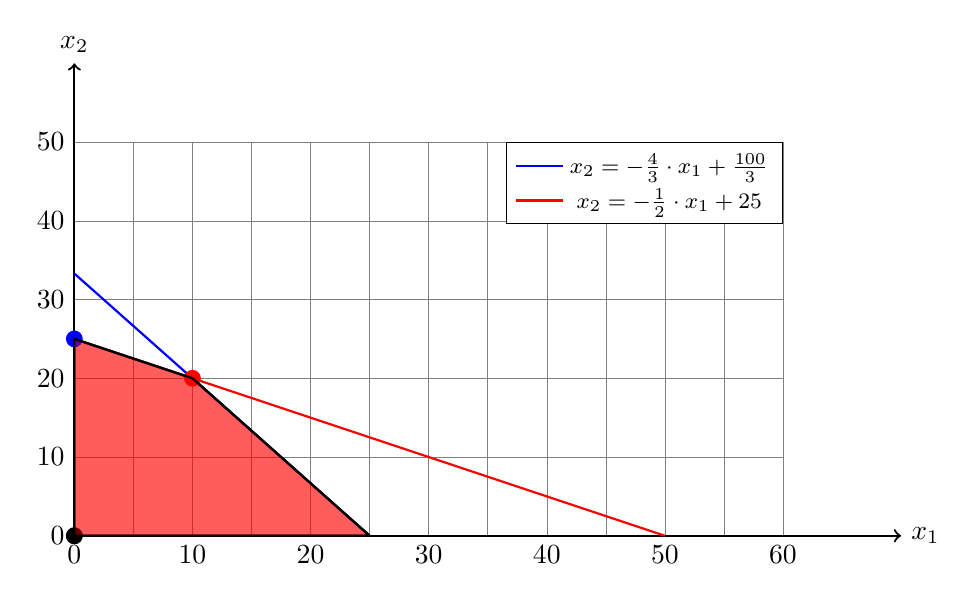
\begin{tikzpicture}[x=0.15cm,y=0.1cm]
		
		\def\xmin{0}
		\def\xmax{60}
		\def\ymin{0}
		\def\ymax{50}
		
		% grid
		\draw[style=help lines, ystep=10, xstep=5] (\xmin,\ymin) grid
		(\xmax,\ymax);
		
		% axes
		\draw[->, thick] (\xmin,\ymin) -- (\xmax+10,\ymin) node[right] {$x_1$};
		\draw[->, thick] (\xmin,\ymin) -- (\xmin,\ymax+10) node[above] {$x_2$};
		
		% xticks and yticks
		\foreach \x in {0,10,...,60}
		\node at (\x, \ymin) [below] {\x};
		\foreach \y in {0,10,...,50}
		\node at (\xmin,\y) [left] {\y};
		
		% plot the data from the file data.dat
		% smooth the curve and mark the data point with a dot
		
		% generate and plot another a curve y = 0.1 x^2 + 2.5
		% this generates the files figure.parabola.gnuplot and figure.parabola.table 
		%\draw[color=red, domain=\xmin:\xmax] plot[id=parabola]
		%function{0.1*x**2 + 2.5} node [right] {$y=0.1\,x^2 + 2.5$};
		\draw [thick, blue](0,33.3) -- (25,0) ;
		\draw [thick, red](0,25) -- (50,0) ;
		
		\node[draw,circle,inner sep=2pt,fill] at (0,0){};
		\filldraw[thick,fill=red,fill opacity=0.4] (0,0) -- (0,25) -- (10,20) -- (25,0) -- (0,0) -- cycle;
		\begin{customlegend}[
			legend entries={ % <= in the following there are the entries
				$ x_2 = -\frac{4}{3}\cdot x_1 + \frac{100}{3} $,
				$x_2 = -\frac{1}{2}\cdot x_1 + 25$
			},
			legend style={at={(60,50)},font=\footnotesize}] % <= to define position and font legend
			% the following are the "images" and numbers in the legend
			\addlegendimage{thick,blue,opacity = 1}
			\addlegendimage{thick,red,opacity = 1}
		\end{customlegend}
		\node[draw,circle,inner sep=2pt,fill] at (0,0){};
		\node[draw,circle,inner sep=2pt,fill,blue] at (0,25){};
		\node[draw,circle,inner sep=2pt,fill, red] at (10,20){};
		
		
		\filldraw[thick,fill=red,fill opacity=0.4] (0,0) -- (0,25) -- (10,20) -- (25,0) -- (0,0) -- cycle;
	\end{tikzpicture}
	\caption{Visualization of the simplified example problem}
	\label{fig:2dvisu}
\end{figure}

\subsubsection{Complexity, Degeneracy and other Properties}
Eventually, we want to briefly discuss the power and the significance of this very algorithm, especially with respect to our original topic, the VEP.\medskip

For bounded, non-\textit{degenerate} polyhedra, the original Simplex algorithm terminates and returns the optimal solution in polynomial time (on average). However, a polyhedron is not always non-degenerate as we will see in the following definition.

\begin{mydef}(Degeneracy)\medskip 
	If a vertex $v$ of $G$ defined by $A,b$ with $m=rank(A)$ solves more than $m$ inequalities as equations, then we will call this vertex \emph{degenerate}. \medskip
	If a polyhedron has at least one degenerate vertex, then we will call this polyhedron \emph{degenerate}.
\end{mydef}

The Simplex method struggles when multiple basic solutions have the same objective value, while also being mutually adjacent. This is the case for degenerate vertices, as we have to interpret one of the basic variables as $0$, too. Thus, multiple states of our Simplex tableau refer to the same vertex, which could lead the algorithm to circle along the basic solutions. However, we can simply introduce an order among the vertices, stating in which sequence they will be chosen, e.g. a lexicographic order of their corresponding basic indices set. This new updating rule is called Bland's rule. Thus, with Bland's rule for pivot selection the Simplex algorithm becomes deterministic and terminates in every case.\medskip

The implications of Bland's rule are discussed in Theorem \ref{Bland}.

\begin{theorem}(Bland's rule)\medskip
	\label{Bland}
	If we use Bland's rule for choosing the Pivot element for the Simplex step, then these updated Simplex steps will always yield a primal feasible basic solution. If Bland's rule is not applicable, then the basic solution is dual feasible and thus optimal.
\end{theorem}

On the other hand, there are much simpler ways to choose a Pivot element. The \textit{Criss-Cross rule} is choosing its row in the Simplex tableau, not by minimizing over the quotients as in \ref{Pivotsel}, but by choosing purely combinatorialy. Thus, the updated Simplex tableau does not always maximize the difference of objective value, contrary to e.g. Bland's rule. 

\begin{lemma}
	\label{theo4}
	If $(P)$ is solvable, then there is a vertex of $G$ which solves $(P)$.
\end{lemma}

Thus, with both rules we will deterministically find the optimal basic solution and its vertex. 

\begin{proposition}
	\label{PropoBland}
	Let $G$ be a polyhedron. If we perform the Simplex algorithm with the update strategy
	\begin{itemize}
		\item Bland's rule, then each generated tableau will be primal feasible and the procedure leads to an optimal basic solution.
		\item Criss-Cross rule, then the procedure leads to an optimal basic solution.
	\end{itemize}
\end{proposition}

Both rules add determinism and thus yield a unique successor for each basic solution $v$. Concatenating the successor edges, we gain a unique path from each basic solution to the optimal one. As this graph is acyclic and connected, these paths build a spanning tree of all vertices of $G$, rooted in the optimal vertex. \medskip

The degeneracy of the optimal vertex however, cannot be immanently solved by neither Bland's or Criss-Cross rule. The graph thus becomes a spanning forest, as the Simplex algorithm stops when reaching an optimal basic solution. Fortunately, we are able to find all optimal basic solutions by a simple search strategy explained later on. If we are given all optimal vertices, we can construct an artificial new vertex, from which all optimal basic solutions are reachable utilizing steps in the dual problem.

\section{The Avis-Fukuda Algorithm}

While these properties of LPs are fairly interesting, how does this help to eventually solve the VEP? Given a polyhedron $G$,  we introduce a random but fixed linear objective function $f(x):=c^Tx$ with $c^T\neq 0$, that defines any gradient along $G$. This leads to the previously mentioned spanning tree of the vertices of $G$. \medskip

It was the idea of Avis and Fukuda, published in the discussed paper, to start a reverse search over this spanning tree to find all vertices, starting from the optimal node. But, the Simplex algorithm only teaches us how to move along the gradient of $f$, and thus only gives as a unidirectional, directed path from any vertex $v$ to the root vertex, but not vice versa. \medskip

\begin{mydef}
	Let $v$ be a basic feasible solution (vertex).\medskip
	
	Let $(\tau, \sigma)$ be the pivot obtained by applying \emph{any} rule to $v$ yielding $v'$.
	We call $(\sigma, \tau)$ the \textit{reverse pivot} for $v'$.
\end{mydef}

By simply pivoting with the same two indices, we can revert a previously done Bland's rule or Criss-Cross rule step. \medskip

This helps us to solve the main issue and major contribution of this paper:\medskip
\begin{quotation}
	Given a vertex $v$, how do we find all vertices $v'$ that have $v$ as its successor?
\end{quotation}
As we can only determine successors and not predecessors of vertices, this problem still remains. Avis and Fukuda were able to resolve this issue by a simple brute force approach: We therefore check all neighbours $v'$ of a given vertex $v$, and check whether Bland's rule takes us back to the original basic solution. In order to do so, we first have to propose the characterization of a neighbour.\medskip

\begin{mydef}(Neighbour)\medskip
	For a given vertex $v$ defined by its set of basic variables $B$, we can define \emph{adjacency} as\medskip
	\begin{equation*}
		Adj(B, i,j) := \left\{ \begin{matrix}
			\emptyset&P_{ij}=0\\
			\emptyset&(B\cup \{i\})-\{j\} \text{ infeasible tableau}\\
			
			(B\cup \{i\})-\{j\}&\text{feasible tableau}
		\end{matrix} \right.
	\end{equation*}
	
	The whole neighbourhood of a vertex is given by
	\begin{equation}
		\textsc{neighbours}(B,N,P):=\{ Adj(B,i.j) | \text{for }i\in N, j\in B\text{ if } Adj(B,i,j)\neq\emptyset \}
	\end{equation}

\end{mydef}

As distinguishing feasible and infeasible tableaus or states is simple, we can easily assemble all feasible neighbours of $v$. We now formulate the above informal description of the procedure in the following algorithm.

\begin{algorithm}[H]
	\caption{Reverse-search the spanning tree}
	\label{alg:seq}
	\begin{algorithmic}[1]
		\STATE \textsc{Search}\textbf{(B,N,P):}
		\FOR{all $i,j$ in \textsc{neighbours}$(B,N,P)$}
		\IF{ \textsc{reverse}$(B,N,P,i,j)$}
		\STATE \textsc{pivot}$(B,N,P,i,j)$
		
		\IF{\textsc{lex\_min}$(B,N,P)$}
		\STATE $print(B)$
		\ENDIF
		\STATE \textsc{Search}$(B,N,P)$
		\STATE \textsc{select-pivot}$(P)$
		\STATE \textsc{pivot}$(B,N,P,i,j)$
		
		\ENDIF
		\ENDFOR
	\end{algorithmic}
\end{algorithm}

The function \textsc{reverse}$(B,N,P,i,j)$ checks  whether $(i,j)$ is a reverse pivot of the state given by $B$. Additionally, we introduce the method \textsc{lex\_min}$(B,N,P)$, which is helpful for the reduction of degenerate vertices. This method checks the current basic solution if it is the minimum with respect to a predefined, lexicographic ordering, among all basic solutions of the current vertex. As the algorithm will visit every basic solution, we thus ensure that the vertex gets printed only once. \textsc{Select-pivot} hereby corresponds to any of the previously mentioned pivoting rules.\medskip 

Starting at the root node, the algorithm checks all adjacent vertices for existence of reverse pivots. If that is the case, the current node gets printed. We then start a recursive search for more vertices from the previously discovered node. While in this algorithm formulation we perform a depth first search, any search technique is viable. If the algorithm has finished the \textsc{search} sub-procedure, it jumps back to its successor with a simple pivoting step. Starting from any first feasible solution, found by usage of the first phase of the Simplex method, we can always find the initial, optimal, root vertex applying the Bland's rule iteratively.\medskip

Eventually, we reached our goal of finding all vertices for our example problem, and are thus free to cook delicious dishes. 

\subsection{Complexity and other properties}
The algorithm gains the following properties derived from the previously described sub-procedures. At first the method does not need any additional storage beyond the input data, as all calculations can be run on the input Simplex tableau. Second, by construction the output will be free of duplicates. Every basic solution will be visited multiple times, but due to the spanning tree and handling of degenerate cases, only output once. Third, the algorithm is extremely simple and requires no complicated data structures, as everything can be computed on the tableau itself. Fourth, the procedure immanently handles all degenerate cases for both optimal and regular tableaus. Regarding time complexity, reverse search is dependent on the amount of vertices, and thus output sensitive for non-degenerate polyhedra and arrangements.
Eventually, given by its recursive search nature and the independence of the subtree searches, the method can be parallelized efficiently and easily.\medskip

Discussing the complexity in more detail, we assume a polyhedron $G\subset\mathbb{R}^d$ with $v$ vertices, bounded by $n$ inequalities. As the dimensionality of $G$ is given by $d$, this is also the amount of necessary non-basic variables. Hence, the Simplex tableau consists of $(n+1)\times (d+1)$ entries added to the constant amount of pointers necessary for the recursion, which reduces to $\mathcal{O}(nd)$ in space complexity. This holds for non-degenerate arrangements, too.\medskip
Observing time complexity, the algorithm has to visit and check all $v$ vertices for the \textsc{reverse} property. As there are $|B|\cdot|N|$ indices pairs for  possible neighbours, we have to repeat the search and revert check $vdn$ times. Hence, the time complexity reduces to $\mathcal{O}(vdn)$ for non-degenerate polyhedra. When including degenerate cases the complexity grows to $\mathcal{O}\left( dn(n+d){n-2\choose d} \right)$. However, for unbounded polyhedra the complexity becomes NP-hard. These bounds also hold for the FEP, given its duality to the VEP.\medskip

Up until now, we treated polyhedra and arrangements similarly, but with respect to time complexity their performance diverges. For a simple, i.e. a non-degenerate, arrangement with $n$ hyperplanes in $\mathbb{R}^d$ and $v$ vertices, we have a complexity of $\mathcal{O}(n^2dv)$. This result corresponds to the degenerate complexity for polyhedra with $v$ substituting ${n\choose d}$, and thus the number of distinct/non-degenerate states checked by \textsc{lex\_min}. We are not able to reduce the complexity further due to the lacking convexity and the multiple possible multiple cells of the given arrangement.

\section{Aftereffects of this publication}

this paper presented not only an approach to three important problems in computational geometry, but also sparked research in many different directions. First, its so fundamental yet so elegant, that it is cited by nearly every book on polyhedra and computational geometry. Second, the authors themselves wrote numerous publications following up this work, as they investigated the reverse search technique (Avis, Fukuda 1996)\cite{AvisReverseSearch} and double description methods (Fukuda, 1995)\cite{FukudaDoubleDescr} in more detail. These publications in return were cited 500 times each. \medskip
 
As Avis and Fukuda's algorithm still remains one of the fastest and most used algorithms for solving VEPs, it was utilized in many different fields and occasions. Adding its immanent ability to be parallelized efficiently, it is implemented in any relevant computational geometry library. Only recently, the VEP and thus the algorithm has experienced an upswing with respect to the field of machine learning, for example in enumerating linear regions.\medskip

As we can see the VEP and the Avis-Fukuda algorithm have been and still are inseparably connected. We thus think that this is one of the most influential papers in computational geometry.


\newpage

\begin{thebibliography}{9}
	\bibitem{introtoAlg} 
	Thomas H. Cormen, Charles E. Leiserson, Ronald L. Rivest und Clifford Stein.
	\textit{Introduction to Algorithms}. Third Edition. The MIT Press, 2009.
	\bibitem{Khachiyan}
	L. Khachiyan, E. Boros, K. Borys, K. Elbassioni, and V. Gurvich. Generating all
	verticesof a polyhedron is hard.Discrete and Computational Geometry,
	39(1):174–190, 2008.
	\bibitem{Motzkin}
	T. S. Motzkin, H. Raiffa, G. L. Thompson, and R. M. Thrall, The Double Description Method,
	Annals of Mathematical Studies, vol. 8, Princeton University Press, Princeton, N J, 1953.
	\bibitem{AvisReverseSearch}
	Avis, D., \& Fukuda, K. (1996). Reverse search for enumeration. Discrete Applied Mathematics, 65(1–3), 21–46. https://doi.org/10.1016/0166-218x(95)00026-n
	\bibitem{FukudaDoubleDescr}
	Fukuda and Prodon, Double Description Method revisited,  Franco-Japanese and Franco-Chinese Conference on Combinatorics and Computer Science, 1995
\end{thebibliography}

\newpage

\section{Appendix}
\subsection*{Visualizations}

In the following we will show the figures illustrating the feasible space. 

\begin{figure}[ht]
	\centering
	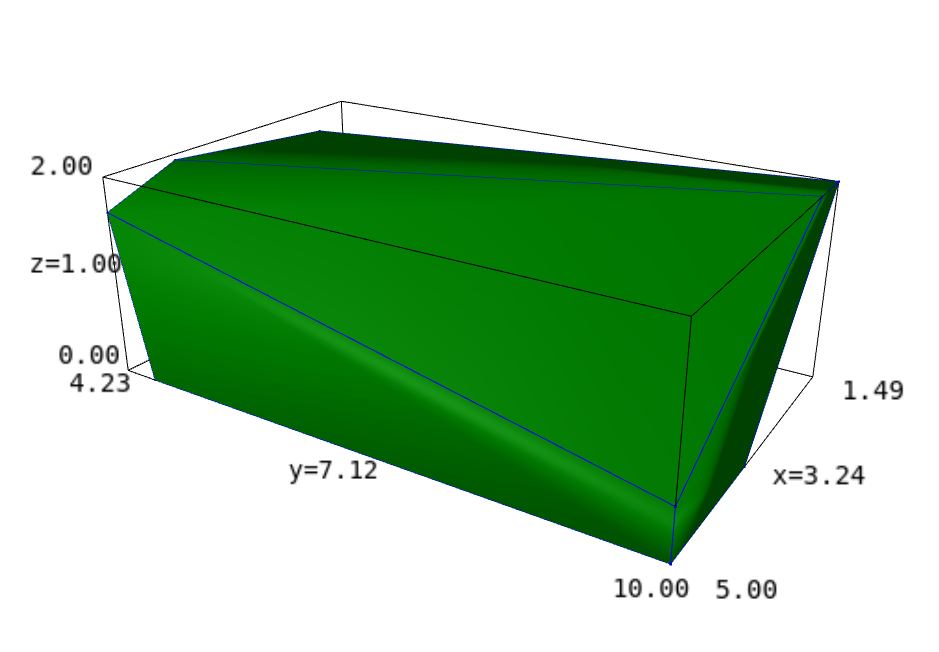
\includegraphics[width = 0.6\textwidth]{../presentation/allMeals2.png}
	\caption{The exact shape is unknown/expensive}
\end{figure}

\begin{figure}[ht]
	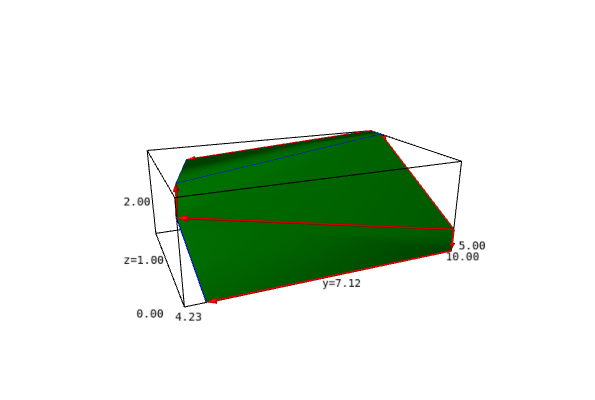
\includegraphics[width = 0.8\textwidth]{../presentation/Polytope_tree.png}
	\caption{The paths span a tree of all vertices}
\end{figure}

\subsection*{Simplex steps}
These are the update rules for a given pivot element $P_{\sigma\tau}$:
\begin{quotation}
	\begingroup
	\def\arraystretch{1.5}
	\begin{tabular}{r|r|r}
		$ST_n$&$x_N$&$1$\\
		\hline
		$x_B=$&$P$&$p$\\
		\hline
		$z=$&$q^T$&$q_0$
	\end{tabular}
	$\longrightarrow$
	\begin{tabular}{r|r|r}
		$ST_{n+1}$&$x_{\bar{N}}$&$1$\\
		\hline
		$x_{\bar{B}}=$&$\bar{P}$&$\bar{p}$\\
		\hline
		$z=$&$\bar{q}^T$&$\bar{q}_0$
	\end{tabular}
	\endgroup
\end{quotation}

\begin{quotation}
	\begingroup
	\def\arraystretch{1.5}
	\begin{tabular}{lrl}
		$I_{\bar{N}} $&$:=$&$ N \backslash\{ \tau \} \cup \{ \sigma \}$\\
		$I_{\bar{B}} $&$:=$&$ B \backslash\{ \sigma \} \cup \{ \tau \}$
	\end{tabular}
	\endgroup
\end{quotation}

\begingroup
\def\arraystretch{2}
\begin{tabular}{p{6.25cm}l}
	\begin{tabular}{lrll}
		$\bar{P}_{\sigma\tau}$&$:=$&$\dfrac{1}{P_{\sigma\tau}} $&\vspace{0.1cm}\\
		$\bar{P}_{\sigma j}$&$:=$&$ -\dfrac{P_{\sigma j}}{P_{\sigma\tau}}$& $ j\in N\ \backslash\{\tau\}$\vspace{0.1cm}\\
		$ \bar{P}_{i\tau}$&$ :=$ & $ \dfrac{P_{i\tau}}{P_{\sigma\tau}} $&$ i\in B\backslash \{\sigma\}$\\
		$ \bar{p}_\sigma $&$:=$&$ -\dfrac{p_\sigma}{P_{\sigma\tau}} $&\\
		$ \bar{p}_i $&$:=$&$ p_i - \dfrac{p_\sigma}{P_{\sigma\tau}}\cdot P_{i\tau}$&$i\in B\backslash\{ \sigma \}$\\
	\end{tabular}&
	\begin{tabular}{lrll}
		$ \bar{q}_\tau $&$:=$&$ \dfrac{q_\tau}{P_{\sigma\tau}} $&\\
		$ \bar{P}_{ij} $&$ := $&$ P_{ij} - \dfrac{P_{\sigma j}}{P_{\sigma\tau}}\cdot q_\tau$&$ i\in B\backslash \{\sigma\}, j\in N\backslash\{\tau\} $\\
		$ q_j $&$ := $&$ q_j - \dfrac{P_{\sigma j}}{P_{\sigma\tau}}\cdot q_\tau $& $ j\in N\backslash\{\tau\} $\\
		$ \bar{q}_0 $&$:=$&$ q_0 - \dfrac{p_\sigma}{P_{\sigma\tau}}\cdot q_\tau $ 
	\end{tabular}
\end{tabular}

\endgroup
\medskip
These are the eventual Simplex steps taken in the reduced example problem:
\begin{quotation}
	
	\begingroup
	\def\arraystretch{2}
	\begin{tabular}{r|rr|r}
		$ST_0$&$x_1$&$x_2$&$1$\\
		\hline
		$x_3=$&$-4$&$-3$&$100$\\
		$x_4=$&$-1$&$-2$&$50$\\
		\hline
		$-z=$&$-30$&$-45$&$0$
	\end{tabular}\hspace{1cm} $\tau = 2, \sigma=4$\\
	\begin{tabular}{r|rr|r}
		$ST_1$&$x_1$&$x_4$&$1$\\
		\hline
		$x_3=$&$-\dfrac{5}{2}$&$\dfrac{3}{2}$&$25$\\
		$x_2=$&$-\dfrac{1}{2}$&$-\dfrac{1}{2}$&$25$\\
		\hline
		$-z=$&$-\dfrac{15}{2}$&$\dfrac{45}{2}$&$-1125$
	\end{tabular}\hspace{1cm} $\tau = 1, \sigma=3$
	\\
	\begin{tabular}{r|rr|r}
		$ST_2$&$x_3$&$x_4$&$1$\\
		\hline
		$x_1=$&$-\dfrac{2}{5}$&$\dfrac{3}{5}$&$10$\\
		$x_2=$&$\dfrac{1}{5}$&$-\dfrac{8}{10}$&$20$\\
		\hline
		$-z=$&$3$&$18$&$-1200$
	\end{tabular}\hspace{1cm} $\longrightarrow$ optimal
	\endgroup
\end{quotation}



\end{document}